%! TEX root = **/000-main.tex
% vim: spell spelllang=en:

\section{Data exploration}%
\label{sec:data-exploration}

\subsection{Pre-processing}%
\label{sub:pre-processing}

As preprocessing, we had to drop all features related to NBA performance except for the target. This is because those metrics will not be available when drafting a new player. Additionally, we had to drop some rows with missing values in the target variable, this happens in case a player is drafted into the NBA but does not play any minutes thus, not recording any stats. We also had to remove some rows corresponding to players that came to the NBA directly after high-score for whom we lack data and other international players from non-well known leagues where no stats had been tracked.

\subsection{Missing values}%
\label{sub:missing-values}

    % df['ts_pct'] = df['ts_pct'].fillna(df['pts_per_g'] / (2*(df['fga_per_g'] + 0.44 * df['fta_per_g'])))
    % df['efg_pct'] = df['efg_pct'].fillna((df['fg_per_g'] + 0.5 * df['fg3_per_g']) / df['fga_per_g'])
    % df['fg3a_per_fga_pct'] = df['fg3a_per_fga_pct'].fillna(df['fg3a_per_g'] / df['fga_per_g'])
    % df['fta_per_fga_pct'] = df['fta_per_fga_pct'].fillna(df['fta_per_g'] / df['fga_per_g'])

We had several columns with missing values, some of them with a high percentage of missing values. We decided to drop any column with more than 50\% missing values.

Features like \texttt{ft\_pct}, \texttt{fg2\_pct}, \texttt{fg3\_pct} which correspond to shot percentages were null when the player had not attempted a shot from that distance. In this case, we considered the best option was to fill these nulls with 0s.

The rest of missing values were imputed using a simple KNN imputation. We believe KNN is a specially good method in this type of data, as players that share some characteristics tend to produce similar stats. \Cref{tab:missing-values} shows the number of imputed
values for each column. Some variables like \texttt{drb\_per\_g}, \texttt{orb\_per\_g} are missing in players drafted before 2001, as at the time these metrics were not tracked. The columns with 130 missing values, are all advanced stats that are not recorded missing in some international leagues.

\begin{table}[htb]
  \centering
  \caption{Imputed Missing values}%
  \label{tab:missing-values}
  \begin{tabular}{llr}
    \toprule
    \textbf{Column} & \textbf{Description} & \textbf{Missing} \\
    \midrule
    \texttt{gs}          & Games Started               & 114 \\
    \texttt{orb\_per\_g} & Offensive Rebounds Per Game & 29  \\
    \texttt{drb\_per\_g} & Defensive Rebounds Per Game & 29  \\
    \texttt{sos}         & Strength of Schedule        & 130 \\
    \texttt{mp}          & Minutes Played              & 130 \\
    \texttt{tov\_pct}    & Turnovers Percentage        & 130 \\
    \texttt{ows}         & Offensive Wins              & 130 \\
    \texttt{dws}         & Defensive Wins              & 130 \\
    \texttt{ws}          & Win Shares                  & 130 \\
    \texttt{ws\_per\_40} & Win Shares Per 40 Minutes   & 130 \\
    \bottomrule
  \end{tabular}
\end{table}

\subsection{Feature selection/extraction}%
\label{sub:feature-selection}

We added some new features like:
\begin{itemize}
    \item \textbf{Age}: Age at which the player was drafted. We used the draft year and player birthday to compute it.
    \item \textbf{Advanced stats:} Several advanced stats were missing for some players, nevertheless we realized that some of them could be computed from the data we had.
    \begin{align*}
    \texttt{efg\_pct} &= \frac{fg + 0.5 * fg3}{fga} & \texttt{ts\_pct} &= \frac{pts}{2*(fgag + 0.44*fta)} \\
    \end{align*}
\end{itemize}

We also performed some feature selection to give us a first insight into which features could be more useful. \Cref{fig:relief} shows the weights obtained using a fast filter method called RReliefF and \cref{fig:pca} shows the results of a sequential forward selection, which gives us a first idea of how many features need to be used.

\begin{figure}[H]
\centering
\begin{minipage}{.5\textwidth}
  \centering
  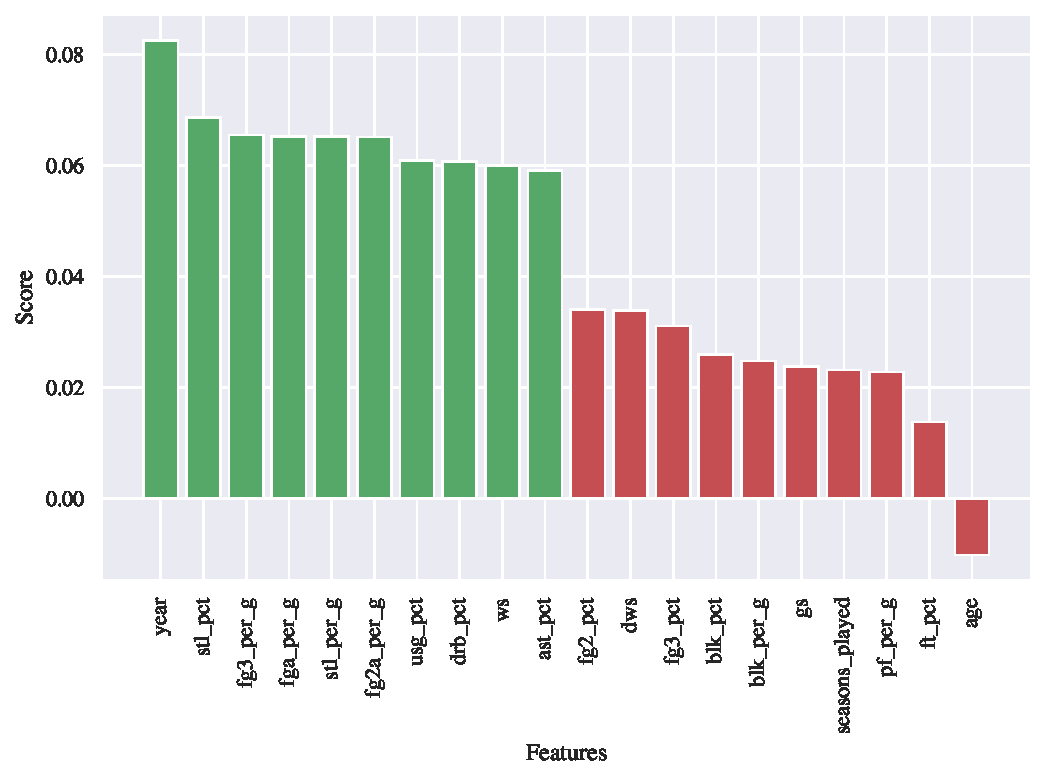
\includegraphics[width=1.0\linewidth]{figures/relief.pdf}
  \captionof{figure}{Top and bottom 10 RReliefF weights}
  \label{fig:relief}
\end{minipage}%
\begin{minipage}{.5\textwidth}
  \centering
  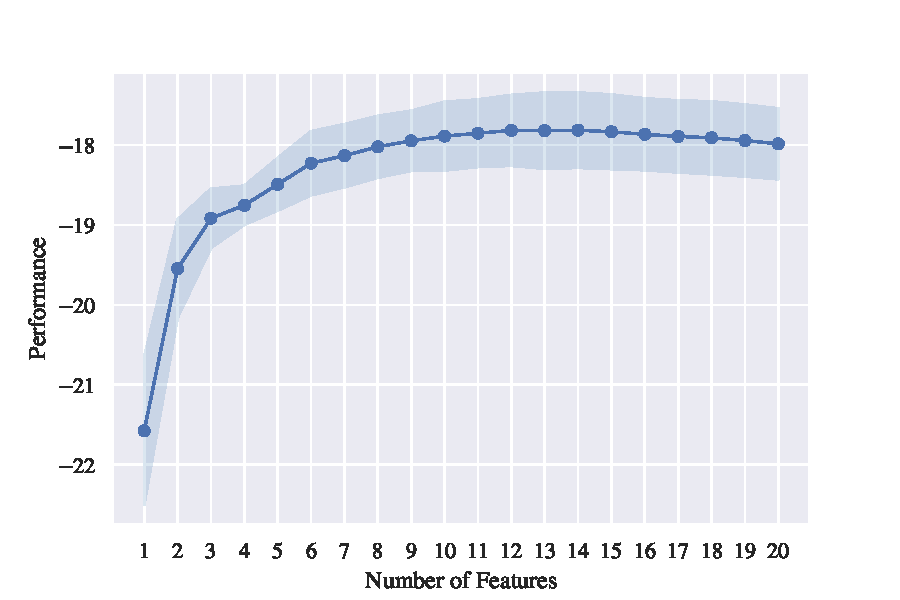
\includegraphics[width=1.0\linewidth]{figures/sfs.pdf}
  \captionof{figure}{SFS score by number of selected features}
  \label{fig:sfs}
\end{minipage}
\end{figure}

\subsection{Visualization}%
\label{sub:visualization}

\subsection{Principal Component analysis}%
\label{sub:pca}

We performed PCA on the data in order to analyze the variance of the data and
consider if we could reduce the dimensionality of the data. \Cref{fig:pca-scree}
shows the scree plot of our PCA. We can see that the first two principal
components account for about 50\% of the variance in our data. With 7
components, we cover 80\% of the variance.

\begin{figure}[H]
  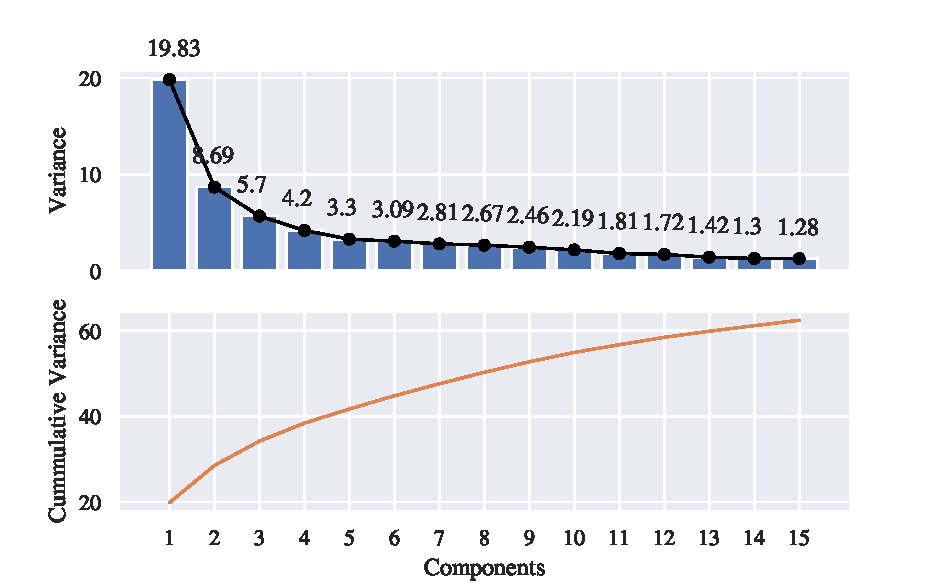
\includegraphics{pca_screeplot}
  \caption{Scree plot for PCA}%
  \label{fig:pca-scree}
\end{figure}

In \cref{fig:pca} we show the projection of the data onto the first two principal
components. There is a slight difference between international players and college ones
in the first axis.

\begin{figure}[H]
  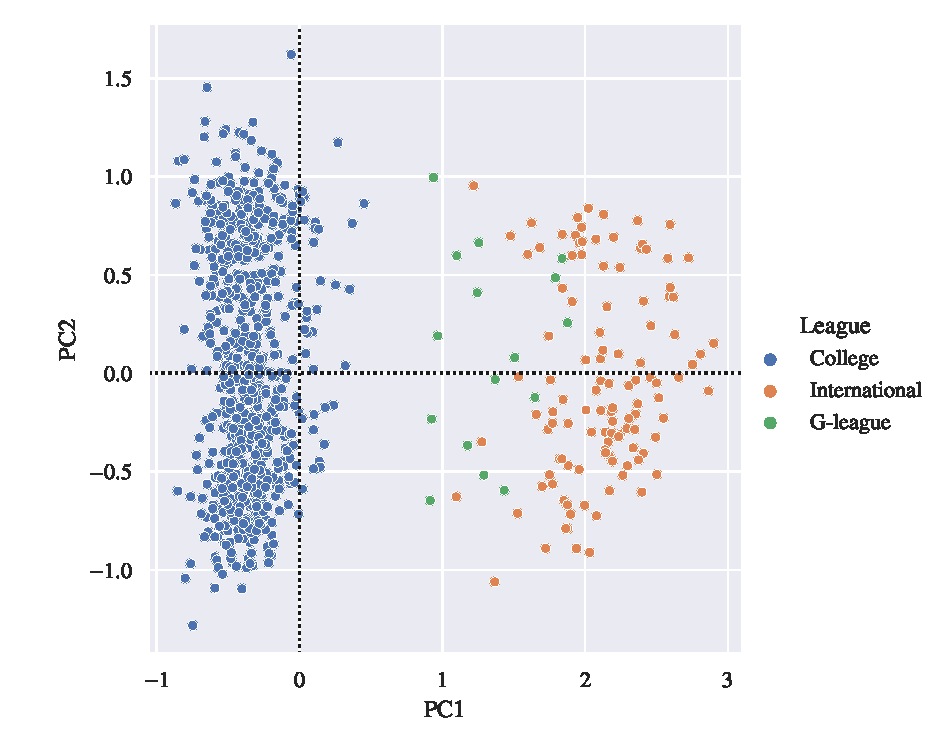
\includegraphics{pca}
  \caption{PCA projection}%
  \label{fig:pca}
\end{figure}

If we analyze the most important features in the first 3 components as shown in
\cref{fig:pca-weights}, we can see that the first component is tightly related
to the 2-point field goals, the second one to the 3-point and the third one to
year.

\begin{table}[htb]
  \centering
  \caption{PCA top features by component}%
  \label{tab:pca-weights}
  \begin{tabular}{clr}
    \toprule
    \makecell{\textbf{Component}\\(variance)}
                         & \textbf{Feature}                                              & \textbf{Weight} \\
    \midrule
    \multirow{5}{*}{\makecell{\textbf{PC1} \\ (28.26\%)}}
                         & Games Started                                                 & -0.317154       \\
                         & 2-Point Field Goal Attempts Per Game                          & -0.272108       \\
                         & Free Throws Per Game                                          & -0.270838       \\
                         & 2-Point Field Goals Per Game                                  & -0.251875       \\
                         & Free Throw Attempts Per Game                                  & -0.247214       \\
                         \midrule
    \multirow{5}{*}{\makecell{\textbf{PC2} \\ (21.62\%)}}
                         & 3-Point Field Goal Attempts Per Game                          & 0.435442        \\
                         & 3-Point Field Goals Per Game                                  & 0.369552        \\
                         & 3-Point Field Goal Attempts Per Field Goal Attempt \%         & 0.362316        \\
                         & Offensive Rebounds Per Game                                   & -0.285247       \\
                         & Blocks Per Game                                               & -0.237038       \\
                         \midrule
   \multirow{5}{*}{\makecell{\textbf{PC3} \\ (9.25\%)}}
                         & Year                                                          & -0.905053       \\
                         & Turnovers Percentage                                          & 0.171122        \\
                         & Defensive Rebounds Per Game                                   & -0.138406       \\
                         & Total Rebounds Per Game                                       & -0.130047       \\
                         & Assists Per Game                                              & 0.129556        \\
    \bottomrule
  \end{tabular}
\end{table}

\subsection{Clustering}%
\label{sub:clustering}

We experimented with several clustering algorithms and transformations on the data. We
found that the only meaningful Clusters we could identify were after scaling the data with
a min-max scaler and transforming it using PCA.
